%!TEX TS-program = xelatex
\documentclass[]{friggeri-cv}
\usepackage{afterpage}
\usepackage{hyperref}
\usepackage{color}
\usepackage{xcolor}
\hypersetup{
    pdftitle={},
    pdfauthor={},
    pdfsubject={},
    pdfkeywords={},
    colorlinks=false,       % no lik border color
   allbordercolors=white    % white border color for all
}
\addbibresource{bibliography.bib}
\RequirePackage{xcolor}
\definecolor{pblue}{HTML}{0395DE}

\begin{document}
\header{Lindsey}{Bennett}
      {Software Designer, Artist}
      
% Fake text to add separator      
\fcolorbox{white}{gray}{\parbox{\dimexpr\textwidth-2\fboxsep-2\fboxrule}{%
.....
}}

% In the aside, each new line forces a line break
\begin{aside}
  \section{Address}
    31 Bolingbroke Street
    Newcastle upon Tyne
    ~
  \section{Tel \& Skype}
    0191 265 5269
    lbennett86
    ~
  \section{Mail}
    \href{mailto:lindsey.bennett@gmail.com}{\textbf{lindsey.bennett}\\gmail.com}
    ~
  \section{Web \& Git}
    \href{http://www.lbennett.net}{lbennett.net}
    \href{https://bitbucket.org/lbennet86}{bitbucket.org/lbennet86}
    \href{https://github.com/lbennet86}{github.com/lbennet86}
    ~
  \section{Programming}
    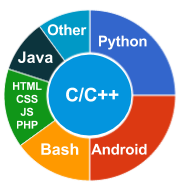
\includegraphics[scale=0.62]{img/programming.png}
    ~
  \section{OS Preference}
    \textbf{GNU/Linux}
\includegraphics[scale=0.40]{img/5stars.png}
    \textbf{Unix}
\includegraphics[scale=0.40]{img/4stars.png}
    \textbf{MacOS}
\includegraphics[scale=0.40]{img/2stars.png}
    \textbf{Windows}
\includegraphics[scale=0.40]{img/1stars.png}
    ~
  \section{Personal Skills}
    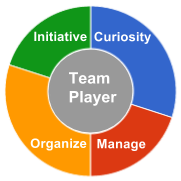
\includegraphics[scale=0.62]{img/personal.png}
    ~
\end{aside}

\section{Experience}
\begin{entrylist}
  \entry
    {03/17 - Now}
    {App Designer, Artist}
    {Weave, Durham UK}
    {Design and implementation of user environment, user experience optimisation, creating art assets for the Weave app.\\}
  \entry
    {01/12 - 02/17}
    {Freelance Developer \& Consultant}
    {Icosaedro Solutions}
    {Design and development of Android Applications, Web Solutions, Unix and GNU/Linux software.\\}
    \entry
    {12/09 - 12/11}
    {Project Manager and Web designer}
    {BBC}
    {Design, development and management of the iPlayer web frontend.\\}
    \entry
    {06/09 - 09/09}
    {Internship}
    {Atitlan Engineering SRL, Pisa, Italy}
    {Management and migration of servers. Development of web templates and interfaces. Management of SQL databases.}
\end{entrylist}

\section{Education}
\begin{entrylist}
  \entry
    {2009 - 2012}
    {Master's Degree in Computer Engineering}
    {Università di Pisa, Italy}
    {Curriculum Networking and Multimedia.\\
    Main subjects: Network Applications, Systems Architecture and Security, Mobile Applications, Multemedia Information            Processing.\\
    \emph{Title of the Thesis: "A Handoff Algorithm based on Link Quality Prediction for Mass Transit Wireless Mesh Networks"      .}\\
    \emph{Relators: Prof. Enzo Mingozzi, Ing. Carlo Vallati, Prof. Luciano Lenzini.}\\}
  \entry
    {2005 - 2009}
    {Bachelor's Degree in Computer Engineering}
    {Università di Pisa, Italy}
    {Main subjects: Matematics and Physics, Programming, Operational Research, Telecommunication Systems, Digital and Analogical Electronics.\\
    \emph{Title of the Thesis: "Development, Management and Migrations of web contents and applications".}\\
    \emph{Thesis activity carried out during an internship period at Atitlan Engineering SRL.}\\}
  \entry
    {2000 - 2005}
    {Scientific Disploma.}
    {Liceo Scientifico, Matera, Italy}
    {Scientific Secondary School.\\
    Main subjects: Mathematics, Physics, Computer Science.}
\end{entrylist}

\section{Certifications}
\begin{entrylist}
  \entry
    {02/2013}
    {Intro to Computer Science}
    {Udacity. E-learning}
    {\emph{Building a Python Search Engine}}
\end{entrylist}

\end{document}
